\section{Thiết kế phương pháp điều khiển dựa trên PPO}
\label{sec:ppo-controller}

\begin{figure}[H]
    \centering
    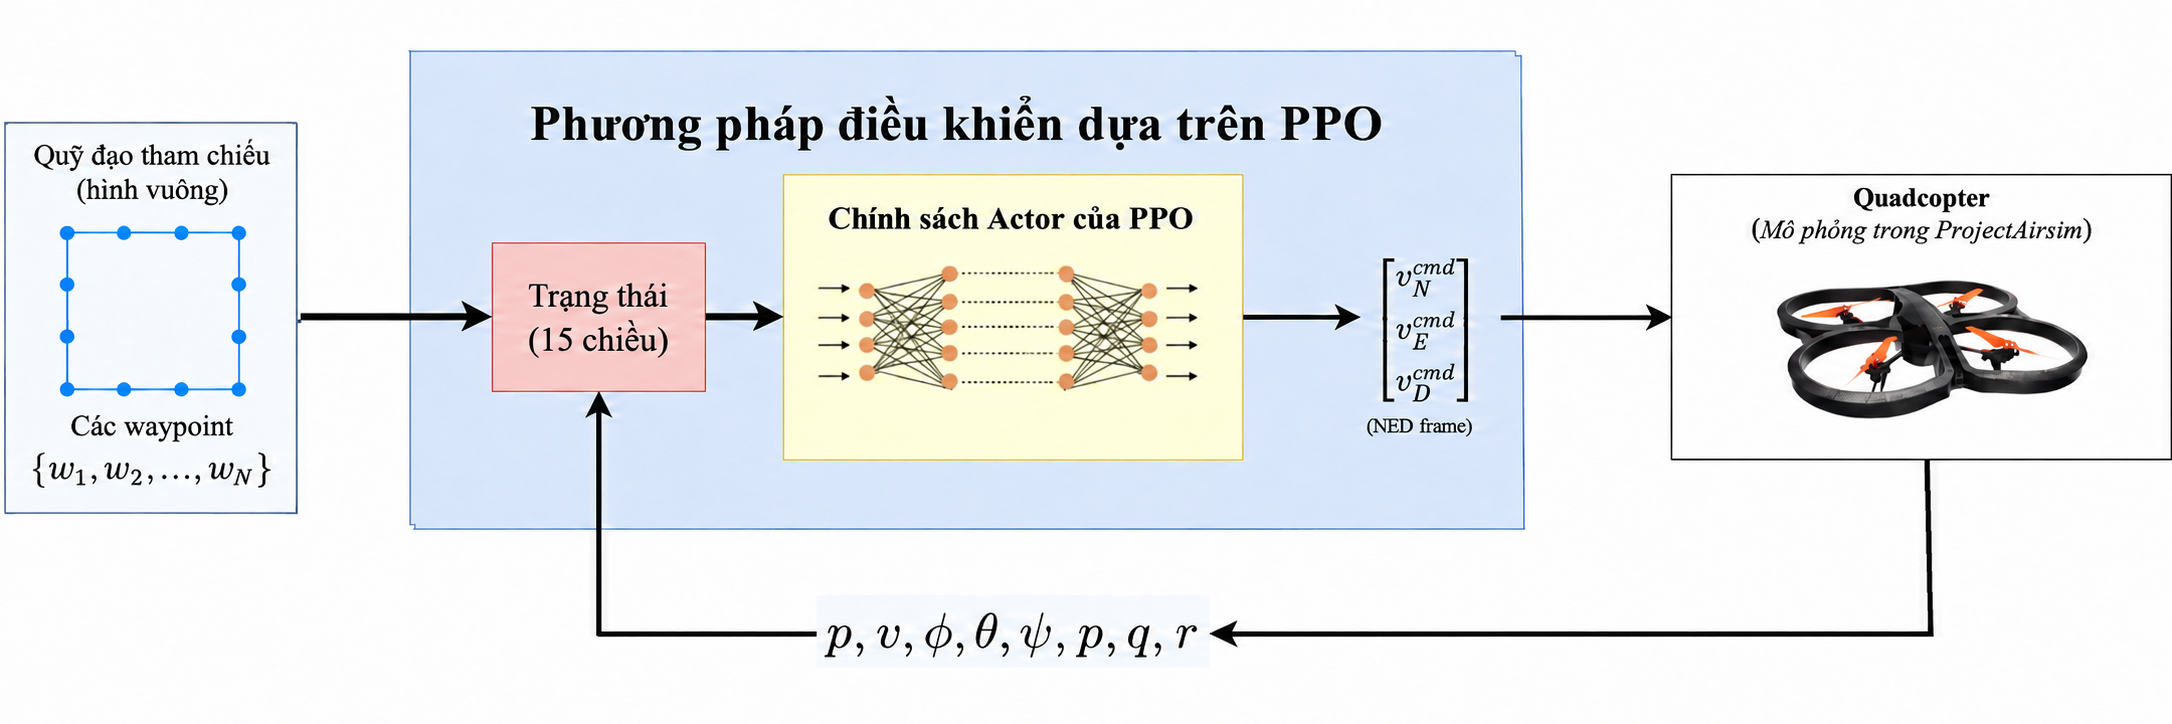
\includegraphics[width=\columnwidth]{Figure/image2-method.png}
    \caption{Kiến trúc điều khiển cho bài toán bám quỹ đạo của quadcopter.}
    \label{fig:ppo-architecture}
\end{figure}

Kiến trúc điều khiển được trình bày trong Hình~\ref{fig:ppo-architecture}. Trong
đó phương pháp điều khiển dựa trên PPO sử dụng thông tin trạng thái của quadcopter và quỹ đạo
tham chiếu làm đầu vào. Chính sách Actor của PPO tính toán và trả về lệnh vận tốc theo hệ tọa độ NED. Các lệnh vận tốc này được truyền tới bộ điều khiển
bay tích hợp trong ProjectAirSim, nơi thực hiện các vòng điều khiển cấp thấp. Trong quá trình hoạt động, các trạng thái chuyển động
gồm vị trí, vận tốc, góc Euler và vận tốc góc sẽ luôn được cập nhật và phản hồi về phương pháp điều khiển dựa trên PPO, từ đó hình thành vòng điều khiển kín.

\subsection{Thiết kế không gian trạng thái}

Không gian trạng thái được thiết kế nhằm cung cấp cho chính sách Actor của PPO các thông tin cần thiết để hoàn thành bài toán. Trạng thái của quadcopter được biểu diễn bởi vectơ

\begin{equation}
\begin{aligned}
\mathbf{s}_t = \bigl[&d_x^i, d_y^i, d_z^i,
 d_x^{i+1}, d_y^{i+1}, d_z^{i+1},\\
 &v_x, v_y, v_z, \phi, \theta, \psi,
 \dot{\phi}, \dot{\theta}, \dot{\psi}\bigr]^{\mathsf{T}}.
\end{aligned}
\label{eq:ppo-state}
\end{equation}

Trong đó:

\begin{itemize}
    \item $d_x^i$, $d_y^i$, và $d_z^i$ là các thành phần của vectơ sai lệch vị trí tương đối từ quadcopter đến waypoint thứ $i$ theo ba trục của hệ tọa độ NED (North--East--Down), được xác định bởi
    \begin{equation}
        \mathbf{d}_i = \boldsymbol{\omega}_i - \mathbf{p}_t,
        \label{eq:relative-position}
    \end{equation}
    trong đó $\mathbf{p}_t = [x, y, z]^{\mathsf{T}} \in \mathbb{R}^3$ là vị trí của quadcopter tại thời điểm $t$, và $\boldsymbol{\omega}_i = [x_{\omega}, y_{\omega}, z_{\omega}]^{\mathsf{T}} \in \mathbb{R}^3$ là vị trí của waypoint thứ $i$;
    \item $d_x^{i+1}$, $d_y^{i+1}$, và $d_z^{i+1}$ là các thành phần của vectơ sai lệch vị trí tương đối từ quadcopter đến waypoint thứ $i+1$;
    \item $v_x$, $v_y$, và $v_z$ là các thành phần vận tốc tuyến tính của quadcopter theo ba trục tọa độ;
    \item $\phi$, $\theta$, và $\psi$ lần lượt là các góc roll, pitch, và yaw mô tả tư thế của quadcopter tại thời điểm $t$;
    \item $\dot{\phi}$, $\dot{\theta}$, và $\dot{\psi}$ là các vận tốc góc quanh các trục roll, pitch, và yaw tương ứng.
\end{itemize}

\subsection{Thiết kế không gian hành động}

Không gian hành động của chính sách Actor của PPO được thiết kế dưới dạng không gian liên tục (continuous action space). Vectơ hành động gồm ba thành phần:

\begin{equation}
    \mathbf{a}_t = \left[v_N^{\mathrm{cmd}}, v_E^{\mathrm{cmd}}, v_D^{\mathrm{cmd}}\right]^{\mathsf{T}}.
    \label{eq:ppo-action}
\end{equation}

Trong đó, $v_N^{\mathrm{cmd}}$, $v_E^{\mathrm{cmd}}$, và $v_D^{\mathrm{cmd}}$ lần lượt là các lệnh vận tốc mong muốn theo ba trục North, East, và Down của hệ tọa độ NED.

Trong nghiên cứu này, chính sách Actor của PPO không trực tiếp gửi lệnh lực đẩy, mô-men điều khiển, hoặc tốc độ quay của từng rotor. Thay vào đó, sau huấn luyện, chính sách Actor tính toán và gửi lệnh vận tốc đến bộ điều khiển bay tích hợp trong ProjectAirSim để điều khiển quadcopter. Trong bài báo, cấu trúc gồm chính sách Actor sinh lệnh vận tốc cấp cao và bộ điều khiển bay tích hợp thực hiện điều khiển cấp thấp được gọi chung là phương pháp điều khiển dựa trên PPO (PPO-based control method).

Để bảo đảm tín hiệu điều khiển nằm trong phạm vi phù hợp, mỗi thành phần hành động được giới hạn bởi

\begin{equation}
    v_N^{\mathrm{cmd}}, v_E^{\mathrm{cmd}}, v_D^{\mathrm{cmd}} \in [-3.0, 3.0]~\mathrm{m/s}.
    \label{eq:action-bound}
\end{equation}

Giới hạn này được triển khai bằng lớp \texttt{Box} của thư viện Gymnasium, bảo đảm rằng các lệnh vận tốc do chính sách Actor của PPO sinh ra không vượt quá phạm vi đã thiết lập trong quá trình huấn luyện và thử nghiệm. Quá trình huấn luyện thuật toán PPO trong môi trường mô phỏng được thực hiện theo cơ chế lock-step với bước thời gian cố định $\Delta t = 0.05$~s, tương ứng với tần số điều khiển $f_c = 1/\Delta t = 20$~Hz.

\subsection{Thiết kế hàm phần thưởng}

Để huấn luyện thuật toán PPO hoàn thành bài toán, hàm phần thưởng gồm bốn thành phần sau:

\begin{equation}
    R_{\mathrm{sum}} = r_{\mathrm{waypoint}} + r_{\mathrm{penalty}} + r_{\mathrm{approach}} + r_{\mathrm{align}}.
    \label{eq:total-reward}
\end{equation}

Trong đó:

\begin{itemize}
    \item $R_{\mathrm{sum}}$ là tổng phần thưởng tại thời điểm $t$;
    \item $r_{\mathrm{waypoint}}$ và $r_{\mathrm{penalty}}$ lần lượt là phần thưởng khi quadcopter hoàn thành waypoint và phạt khi quadcopter vi phạm điều kiện an toàn.;
    \item $r_{\mathrm{approach}}$ là phần thưởng tiếp cận waypoint, khuyến khích quadcopter giảm khoảng cách tới waypoint hiện tại;
    \item $r_{\mathrm{align}}$ là phần thưởng liên tục khuyến khích quadcopter duy trì hướng chuyển động thẳng hàng với hướng từ vị trí quadcopter đến waypoint.
\end{itemize}

\subsubsection{Phần thưởng hoàn thành waypoint}

Để khuyến khích quadcopter hoàn thành các waypoint theo đúng thứ tự trên quỹ đạo tham chiếu, phần thưởng có dạng như sau:
\begin{equation}
 r_{\mathrm{waypoint}} =\!
 \begin{cases}
  10, & d(\mathbf{p}_t, \boldsymbol{\omega}_i) < r_{\omega},\ i < n,\\[4pt]
  15\left(1 + \displaystyle\frac{T_{\max}-t}{T_{\max}}\right),
      & d(\mathbf{p}_t, \boldsymbol{\omega}_i) < r_{\omega},\ i = n,\\[8pt]
  0, & \text{ngược lại}.
 \end{cases}
 \label{eq:waypoint-reward}
\end{equation}

Trong đó, $\mathbf{p}_t \in \mathbb{R}^3$ là vị trí của quadcopter tại thời điểm $t$, $\boldsymbol{\omega}_i \in \mathbb{R}^3$ là waypoint thứ $i$, $T_{\max}$ là số bước tối đa của một episode, $r_{\omega}$ là bán kính xác định quadcopter hoàn thành waypoint, và
$d(\mathbf{p}_t, \boldsymbol{\omega}_i)= \left\|\mathbf{p}_t - \boldsymbol{\omega}_i\right\|_2$
là khoảng cách Euclid giữa quadcopter và waypoint mục tiêu. Quadcopter được xác định là đã hoàn thành waypoint mục tiêu khi $d(\mathbf{p}_t, \boldsymbol{\omega}_i) < r_{\omega}$. Khi quadcopter đến waypoint trung gian, hàm phần thưởng trả về một giá trị dương. Nếu quadcopter hoàn thành waypoint cuối cùng trước khi hết số bước tối đa của episode, hàm phần thưởng trả về thêm phần thưởng phụ thuộc vào số bước thời gian còn lại.

\subsubsection{Phạt vi phạm điều kiện an toàn}

Tại mỗi bước thời gian, nếu episode kết thúc sớm do quadcopter va chạm với mặt đất, bị lật, hoặc cách waypoint mục tiêu quá xa, thuật toán PPO nhận một giá trị phạt âm lớn trong quá trình huấn luyện:

\begin{equation}
    r_{\mathrm{penalty}} = -30.
    \label{eq:safety-penalty}
\end{equation}

Cơ chế này được xem như một ràng buộc an toàn, giúp cho quadcopter tránh được các tình huống nguy hiểm như chạm mặt đất, bị lật khi $|\phi|$ hoặc $|\theta| > \pi/2$, hoặc di chuyển quá xa so với waypoint mục tiêu. 
Việc sử dụng cùng một mức phạt lớn cho các sự kiện nguy hiểm nhấn mạnh rằng mọi tình huống làm episode kết thúc sớm đều không mong muốn và cần tránh trong quá trình bay. Nếu không xuất hiện sự kiện nguy hiểm, quá trình huấn luyện tiếp tục kiểm tra điều kiện đạt waypoint.

\subsubsection{Phần thưởng tiếp cận waypoint}

Phần thưởng tiếp cận waypoint $r_{\mathrm{approach}}$ được xác định như sau:

\begin{equation}
 r_{\mathrm{approach}} = \max\left\{0,\;5.0\left[
 d(\mathbf{p}_{t-1}, \boldsymbol{\omega}_i)
 - d(\mathbf{p}_t, \boldsymbol{\omega}_i)
 \right]\right\}.
 \label{eq:progress-reward}
\end{equation}

Trong đó, $d(\mathbf{p}_{t-1}, \boldsymbol{\omega}_i)$ và $d(\mathbf{p}_t, \boldsymbol{\omega}_i)$ lần lượt là khoảng cách từ quadcopter đến waypoint thứ $i$ tại các thời điểm $t-1$ và $t$. Phần thưởng tiếp cận waypoint $r_{\mathrm{approach}}$ được thiết kế nhằm khuyến khích quadcopter giảm khoảng cách tới waypoint hiện tại sau mỗi bước thời gian. Theo đó, thành phần này nhận giá trị dương khi khoảng cách tới waypoint hiện tại giảm so với bước thời gian trước; ngược lại, thành phần này bằng $0$ khi quadcopter không tiến gần waypoint.

\subsubsection{Phần thưởng hiệu chỉnh vận tốc}

Thành phần $r_{\mathrm{align}}$ khuyến khích quadcopter duy trì hướng chuyển động thẳng hàng với hướng từ vị trí hiện tại đến waypoint. Phần thưởng có dạng như sau:
\begin{equation}
 r_{\mathrm{align}} = \max\left\{0,\;0.2\,\mathbf{v}_t \cdot
 \frac{\boldsymbol{\omega}_i - \mathbf{p}_t}
 {d(\mathbf{p}_t, \boldsymbol{\omega}_i)}\right\}.
 \label{eq:alignment-reward}
\end{equation}

Trong đó $\mathbf{v}_t \in \mathbb{R}^3$ là vectơ vận tốc tuyến tính của quadcopter tại thời điểm $t$. Giá trị phần thưởng là tích vô hướng giữa vectơ vận tốc và vectơ đơn vị hướng tới waypoint. Thành phần này nhận giá trị dương khi vectơ vận tốc có thành phần hướng về waypoint, tương ứng với góc giữa hai vectơ nhỏ hơn $90^\circ$. Khi quadcopter bay vuông góc hoặc theo hướng rời xa waypoint, phần thưởng bằng $0$.

\subsection{Mạng Actor--Critic}

Thuật toán Proximal Policy Optimization (PPO)~\cite{b20} được huấn luyện với kiến trúc Actor--Critic. Trong quá trình huấn luyện, mạng Actor thực hiện ánh xạ trạng thái hiện tại của quadcopter thành lệnh vận tốc mong muốn, trong khi mạng Critic ước lượng giá trị của trạng thái nhằm hỗ trợ quá trình cập nhật chính sách. Sau huấn luyện, chính sách Actor của PPO được triển khai trong phương pháp điều khiển dựa trên PPO để sinh lệnh vận tốc NED.

Cả Actor và Critic đều nhận vectơ trạng thái \(\mathbf{s}_t \in \mathbb{R}^{15}\) được xác định trong Phần~\ref{sec:problem-formulation} làm đầu vào. Trước khi đưa vào mạng, các thành phần trạng thái được chuẩn hóa nhằm hạn chế ảnh hưởng của sự khác biệt về thang đo giữa các biến quan sát. Mỗi mạng gồm hai lớp ẩn fully connected, mỗi lớp có 64 nơ-ron và sử dụng hàm kích hoạt Tanh.

